\documentclass[a4paper,11pt,DIV14,BCOR0mm]{scrartcl}
\usepackage[utf8]{inputenc}
\usepackage[francais]{babel}
\usepackage[T1]{fontenc}
\usepackage{amsmath}
\usepackage{amssymb}
\usepackage{color}
\usepackage{textcomp}
\usepackage[official]{eurosym}
\usepackage{enumitem}
\usepackage{numprint}
\usepackage{graphicx}
\usepackage{xifthen}
\usepackage{pifont}
%\usepackage{xlop}
\usepackage{subfig}
\usepackage{cellspace,stmaryrd}
\usepackage[french]{varioref}
\usepackage{pstricks,pst-circ,pstricks-add,pst-plot,pst-math}
%\usepackage{pst-all,pst-tree,pst-3dplot}
\RequirePackage[amsmath,thmmarks,hyperref,framed]{ntheorem}
\usepackage{mathrsfs}

% ==================================================
% Intervalles
% ==================================================
\newcommand{\intervalle}[4]{\mathopen{#1}#2\mathpunct{};#3\mathclose{#4}}
\newcommand{\intff}[2]{\intervalle{[}{#1}{#2}{]}}
\newcommand{\intof}[2]{\intervalle{]}{#1}{#2}{]}}
\newcommand{\intfo}[2]{\intervalle{[}{#1}{#2}{[}}
\newcommand{\intoo}[2]{\intervalle{]}{#1}{#2}{[}}
\newcommand{\intn}[2]{\intervalle{\llbracket}{#1}{#2}{\rrbracket}}
\newcommand{\bigintervalle}[4]{\bigl{#1}#2\mathpunct{};#3\bigr{#4}}
\newcommand{\bigintff}[2]{\bigintervalle{[}{#1}{#2}{]}}
\newcommand{\bigintof}[2]{\bigintervalle{]}{#1}{#2}{]}}
\newcommand{\bigintfo}[2]{\bigintervalle{[}{#1}{#2}{[}}
\newcommand{\bigintoo}[2]{\bigintervalle{]}{#1}{#2}{[}}
\newcommand{\bigintn}[2]{\bigintervalle{\llbracket}{#1}{#2}{\rrbracket}}
\newcommand{\Bigintervalle}[4]{\Bigl{#1}#2\mathpunct{};#3\Bigr{#4}}
\newcommand{\Bigintff}[2]{\Bigintervalle{[}{#1}{#2}{]}}
\newcommand{\Bigintof}[2]{\Bigintervalle{]}{#1}{#2}{]}}
\newcommand{\Bigintfo}[2]{\Bigintervalle{[}{#1}{#2}{[}}
\newcommand{\Bigintoo}[2]{\Bigintervalle{]}{#1}{#2}{[}}
\newcommand{\Bigintn}[2]{\Bigintervalle{\llbracket}{#1}{#2}{\rrbracket}}
\newcommand{\biggintervalle}[4]{\biggl{#1}#2\mathpunct{};#3\biggr{#4}}
\newcommand{\biggintff}[2]{\biggintervalle{[}{#1}{#2}{]}}
\newcommand{\biggintof}[2]{\biggintervalle{]}{#1}{#2}{]}}
\newcommand{\biggintfo}[2]{\biggintervalle{[}{#1}{#2}{[}}
\newcommand{\biggintoo}[2]{\biggintervalle{]}{#1}{#2}{[}}
\newcommand{\biggintn}[2]{\biggintervalle{\llbracket}{#1}{#2}{\rrbracket}}
\newcommand{\Biggintervalle}[4]{\Biggl{#1}#2\mathpunct{};#3\Biggr{#4}}
\newcommand{\Biggintff}[2]{\Biggintervalle{[}{#1}{#2}{]}}
\newcommand{\Biggintof}[2]{\Biggintervalle{]}{#1}{#2}{]}}
\newcommand{\Biggintfo}[2]{\Biggintervalle{[}{#1}{#2}{[}}
\newcommand{\Biggintoo}[2]{\Biggintervalle{]}{#1}{#2}{[}}
\newcommand{\Biggintn}[2]{\Biggintervalle{\llbracket}{#1}{#2}{\rrbracket}}

\newcommand{\pt}{.}
\newcommand{\et}{\text{ et }}
\newcommand{\si}{\text{ si }}
\newcommand{\tq}{\text{ tq }}
\newcommand{\sinon}{\text{ sinon }}
\newcommand{\avec}{\text{ avec }}
\def\pour{\text{~pour~}}

\newenvironment{enumeratecol}[1][2]{\begin{multicols}{#1}\begin{enumerate}}{\end{enumerate}\end{multicols}}


\newcommand{\set}[1]{\left\{#1\right\}}


%\newtheorem{theoreme}{Théorème}
%\newtheorem{axiome}{Axiome}
\newtheorem*{proprieteadmise}{Propriété (admise)}
%\newtheorem*{demonstration}{Démonstration}
\newtheorem*{notation}{Notation}
\newtheorem*{application}{Application}
\newtheorem*{consequence}{Conséquence}
\newtheorem{roc}{Restitution organisée de connaissances.}


\theoremstyle{plain}
\theoremheaderfont{\normalfont\bfseries}
\theorembodyfont{\normalfont}
\theoremseparator{.}
\newtheorem{exercice}{Exercice}
\newtheorem{cours}{Question de cours}
\newtheorem{probleme}{Problème}

\theoremstyle{plain}
\theoremheaderfont{\normalfont\bfseries}
\theorembodyfont{\normalfont}
\theoremseparator{.}
\newtheorem*{rappel}{Rappel}
\newtheorem{exemple}{Exemple}
\newtheorem*{contreexemple}{Contre-exemple}
\newtheorem{remarque}{Remarque}
\newtheorem*{interpretation}{Interprétation}
\newtheorem*{convention}{Convention}
\newtheorem*{vocabulaire}{vocabulaire}

\theoremheaderfont{\sc}\theorembodyfont{\upshape}
\theoremstyle{nonumberplain}
\theoremseparator{ : }
%\theoremsymbol{\rule{1ex}{1ex}}
\theoremsymbol{\ensuremath\square}
\newtheorem{demonstration}{D\'emonstration}



\usepackage[S]{thmbox}
\newtheorem[S]{theoreme}{Théorème}
\newtheorem[S]{propriete}{Propriété}
\newtheorem[S]{axiome}{Axiome}
\newtheorem[S]{methode}{Méthode de résolution}
\newtheorem[L]{definition}{Définition}

\newcommand{\defi}[1]{
\begin{definition}
#1
\end{definition}
}

\newcommand{\theo}[1]{
\begin{theoreme}
#1
\end{theoreme}
}

\newcommand{\demo}[1]{
\begin{demonstration}
#1
\end{demonstration}
}


%-------------------------------------------------
%         TYPOGRAPHIE
%-------------------------------------------------
\newcommand{\celsius}{\,\degres\textrm{C}}


%-------------------------------------------------
%         SCOLAIRE
%-------------------------------------------------
\newcommand{\trou}[1]{\textcolor{white}{#1}}
\newcommand{\prof}[1]{\textcolor{blue}{#1}}
\newcommand{\exercices}[1]{\begin{flushright}\textbf{Exercices : }#1\end{flushright}}

\newcommand{\np}[1]{\numprint{#1}}

\newcommand{\place}[1]{
\vfill\begin{center}
< #1>
\end{center}
\vfill
}

\newif\ifeleve
\def\ac#1{\ifeleve%
\setbox1\hbox{#1}%
\lower2pt\hbox to \wd1{\dotfill}%
\else#1\fi}

\newcommand{\croi}{% croissante
\unitlength=1cm
\begin{minipage} {1cm}%pour centrer verticalement f(x)
\begin{picture}(1,1) % dessin de 2 X 2
\put(0,0){\vector(1,1){1}} % 1 à partir (0,0) direction (1,1)
\end{picture}
\end{minipage}
}
\newcommand{\dec}{%décroissante
\unitlength=1cm
\begin{minipage} {1cm}%pour centrer verticalement f(x)
\begin{picture}(1,1) % dessin de 2 X 2
\put(0,1){\vector(1,-1){1}}
\end{picture}
\end{minipage}
} 

\newcommand{\tauxfxh}[3]{\dfrac{#1(#2+#3)-#1(#2)}{#3}}

\newcounter{QCM}
\setcounter{QCM}{1}
\newcommand{\question}[1]{{\item[Question \arabic{QCM}]\addtocounter{QCM}{1}#1}}
\newcommand{\choix}[3]{
\[
 \begin{tabular}{p{5cm}p{5cm}p{5cm}}
  \textbf{a) }#1.&\textbf{b) }#2.&\textbf{c) }#3.
 \end{tabular}
\]
}

%-------------------------------------------------
%         GEOMETRIE
%-------------------------------------------------
\newcommand{\vect}{\overrightarrow}
\newcommand{\norme}[1]{\|#1\|}
\newcommand{\Norme}[1]{\left\|#1\right\|}
\newcommand{\Oijk}{(O,\vect{i},\vect{j},\vect{k})}
\newcommand{\Oij}{(O,\vect{i},\vect{j})}
\newcommand{\Ouv}{(O,\vect{u},\vect{v})}
\newcommand{\bary}{\mathrm{Bar}}

%-------------------------------------------------
%         FONCTIONS
%-------------------------------------------------
\newcommand{\donne}{\mapsto}
\newcommand{\dx}{\mathrm{d}x}
\newcommand{\dt}{\mathrm{d}t}
\newcommand{\intab}{\int_{a}^{b}}
%-------------------------------------------------
%         PROBA
%-------------------------------------------------
\newcommand{\barre}[1]{\overline{#1}}

%-------------------------------------------------
%         ALGEBRE LINEAIRE
%-------------------------------------------------
\newcommand{\rg}{\text{rg}}
\newcommand{\tr}{\text{tr}}
\renewcommand{\Im}{\text{Im}}
\newcommand{\Vect}{\text{Vect}}
\newcommand{\LL}{\mathcal{L}}
\newcommand{\FF}{\mathcal{F}}
\newcommand{\MM}{\mathcal{M}}
\newcommand{\transpose}{{}^{t}}
%\newcommand{\ker}{\text{ker}}
\newcommand{\coordo}[2]{
\begin{pmatrix}
#1 \\ #2
\end{pmatrix}
}

%-------------------------------------------------
%         ARITHMETIQUE
%-------------------------------------------------
\newcommand{\congru}{\equiv}

%-------------------------------------------------
%         NOMBRES COMPLEXES
%-------------------------------------------------
\newcommand{\e}{\mathrm{e}}
\newcommand{\ii}{\mathrm{i}}
\newcommand{\ei}[1]{\mathrm{e}^{\ii#1}}
\newcommand{\C}{\mathbb{C}}
\newcommand{\U}{\mathbb{U}}
\newcommand{\re}[1]{\mathrm{Re}(#1)}
\newcommand{\im}[1]{\mathrm{Im}(#1)}
\newcommand{\conj}[1]{\overline{#1}}
\newcommand{\abs}[1]{\left\lvert#1\right\rvert}
\renewcommand{\arg}[1]{\mathrm{Arg}(#1)}

\newcommand{\pparmin}[2]{\binom{#2}{#1}}
\newcommand{\Pparmin}[2]{\dbinom{#2}{#1}}

\newcommand{\R}{\mathbb{R}}
\newcommand{\K}{\mathbb{K}}
\newcommand{\N}{\mathbb{N}}
\newcommand{\Z}{\mathbb{Z}}
\newcommand{\D}{\mathbb{D}}
\newcommand{\Q}{\mathbb{Q}}
\newcommand{\rond}{\circ}
\newcommand{\repereoij}{repère orthonormal $(O,\vect{i},\vect{j})$}
\newcommand{\repereoijdirect}{repère orthonormal direct $(O,\vect{i},\vect{j})$}
\newcommand{\accoladedouble}[2]{\left\{\begin{array}{ll}#1\\#2\end{array}\right.}
\newcommand{\soitlasuite}[4]{Soit $(#1)$ la suite définie par $\accoladedouble{#2}{#3\text{ pour tout $#4$}}$}
\newcommand{\coordvect}[2]{\left(\begin{array}{c}#1\\#2\end{array}\right)}
\newcommand{\baremeexo}[1]{\marginpar{\textbf{(#1)}}}
\newcommand{\baremeque}[1]{\marginpar{(#1)}}
\newcommand{\bq}[1]{\marginpar{\textcolor{red}{(#1)}}}


\newcommand{\less}{\leqslant}
\newcommand{\more}{\geqslant}
\newcommand{\equi}{\Longleftrightarrow}
\newcommand{\implique}{\Rightarrow}
\newcommand{\equidef}{\stackrel{def}{\Longleftrightarrow}}
\newcommand{\ssi}{\Longleftrightarrow}
\newcommand{\eqdef}{\stackrel{def}{=}}
\newcommand{\egaldef}{\stackrel{\tiny{def}}{=}}
\newcommand{\egalnot}{\stackrel{\tiny{notation}}{=}}
\newcommand{\latin}[1]{\emph{#1}}
\newcommand{\negl}[1]{\underset{\text{\tiny{$#1$}}}{\ll}}

\newcommand{\limsuite}{\displaystyle\lim_{n\to+\infty}}

% Partie à ommettre en première lecture
\newcommand{\optionnel}[1]{\noindent\hrulefill \rotatebox{180}{\ding{72}\ding{72}\ding{72}} \hrulefill #1 \noindent\hrulefill \ding{72}\ding{72}\ding{72} \hrulefill}
% En tête et pieds custom
\usepackage{fancyhdr}
\pagestyle{fancy}
\lhead{\today}
\rhead{Cours}		
\lfoot{\tiny{vg}}
\cfoot{}
\rfoot{\tiny{Lycée Émile Loubet, Valence}}


% de Dupuy de lome
%\newcommand{\norme}[1]{\left\lVert\ifempty{#1}{\dotpourvariable}{#1}\right\rVert}
\newcommand{\bignorme}[1]{\bigl\lVert#1\bigr\rVert}
\usepackage{hyperref}
\rhead{Septembre 2012}
\chead{}
\lhead{Exercices sur les suites}
\lfoot{\tiny{vg}}
\cfoot{\thepage}
\rfoot{\tiny{Julie-Victoire Daubié, Argenteuil, TS2}}
\begin{document}
\section{Définitions explicites, définitions par récurrence}


\begin{exercice}
 Pour les suites suivantes, écrire les 2 \og définitions\fg{} équivalentes non données parmi les
3 : avec $\cdot$, avec $\sum$, par récurrence. Calculer les 3 premiers termes de la suite.
\begin{itemize}
  \item Pour $n\geq1$, $U_n=1+\dfrac{1}{4}+\dfrac{1}{9}+\cdots+\dfrac{1}{n^2}$.
  \item Pour $n\geq1$, $V_n=\sum_{k=1}^n k^3$.
  \item $W_1=1$ et pour $n\geq2$, $W_{n}=W_{n-1}+\dfrac{1}{n}$.
  \item Pour $n\geq1$, $g_n=2n-1$ et $G_n=\sum_{k=1}^{n}g_k$.
À propos, ce texte de Galilée cité dans le sujet de Physique du bac S 2011 :
\[
 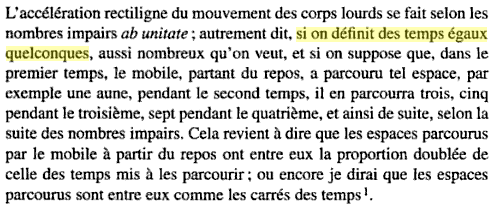
\includegraphics[width=0.5\textwidth]{galilee.png}
\]
\end{itemize}
\end{exercice}


\begin{exercice}
 Pour chacune des suites mal définies en introduction, donner si possible une définition par récurrence et une définition explicite.
\end{exercice}


Pour les suites arithmétiques et géométriques, le passage de la définition par
récurrence à une expression explicite est connu et simple.
\pagebreak
\section{Suites arithmétiques, suites géométriques}

\[
 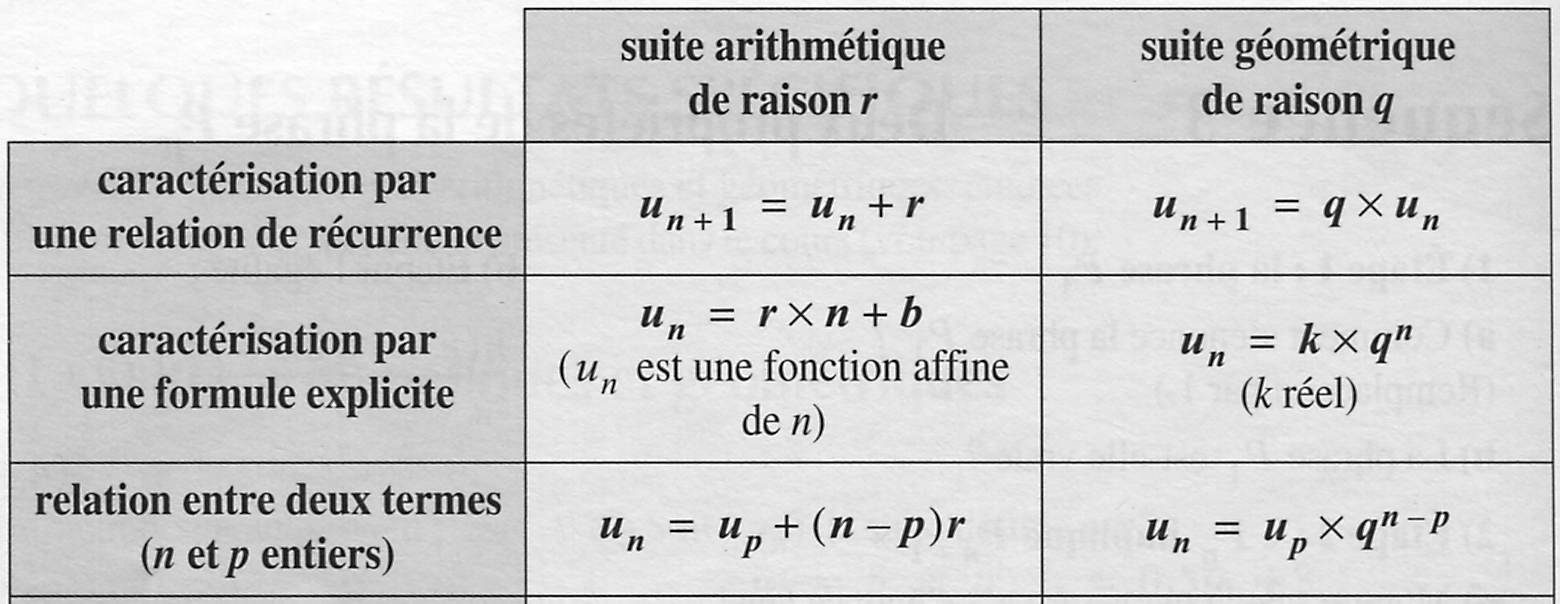
\includegraphics{rappels_terracher}
\]
\begin{center}
 Extrait du manuel Terracher, TaleS
\end{center}

\begin{exemple}
 On place un capital $K_0=\numprint{100}$ à 5\%. On note $K_n$ le capital acquis
l'année $n$. $(K_n)_{n\in\N}$ est la suite géométrique de terme initial $K_0=100$
et de raison 1,05. On a :
\begin{align*}
 K_0&=100\\
 K_1&=1,05\times100=105\\
 K_2&=1,05\times105=110.25=1,05^2\times100\\
 K_3&=1,05\times110,25=\numprint{115,7625}=1,05^3\times100\\
\dots
\end{align*}
\end{exemple}

\begin{theoreme}[Somme de termes consécutifs d'une suite arithmétique]
Soit $p\geq n$, dans les hypothèses de la définition d'une suite arithmétique on a :
 \[
  \sum_{k=n}^{p}u_k=u_n+u_{n+1}+\dots+u_{p}=(p-n+1)\frac{u_n+u_p}{2}.
 \]
\end{theoreme}
 On admet ce théorème. L'idée d'une preuve repose sur le dessin ci-après, l'aire du rectangle
est le double de la somme cherchée :
\[
 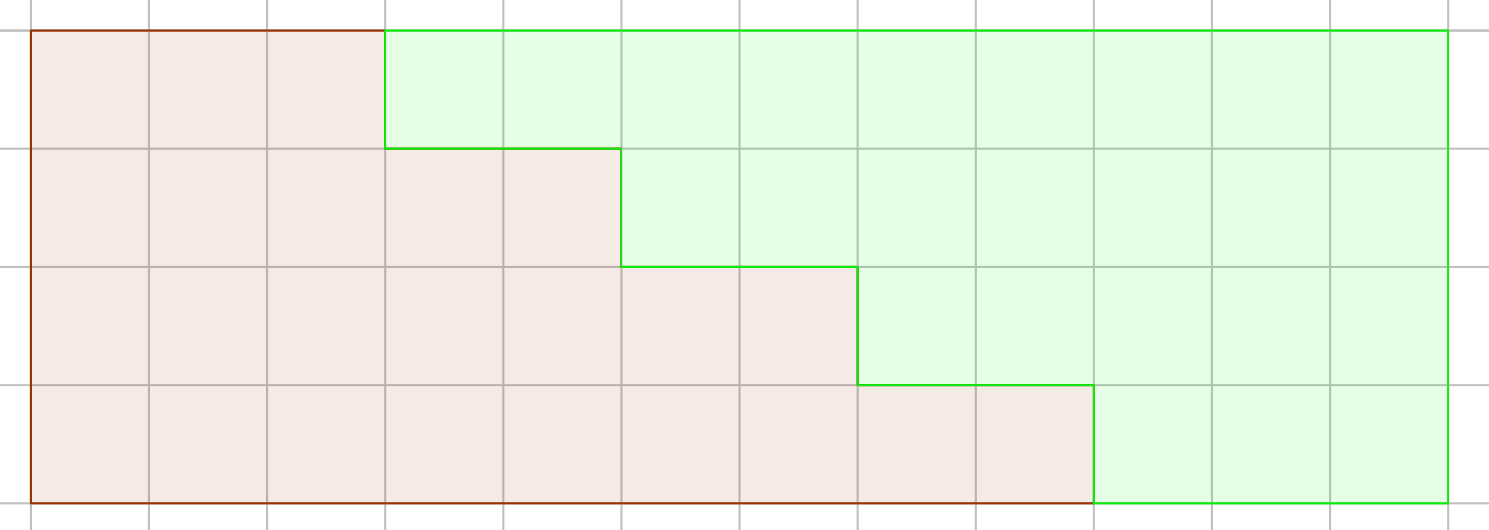
\includegraphics[width=0.5\textwidth]{seriearithmetique}
\]
\begin{theoreme}[Culture générale, jolie formule]
Pour tout $n\in\N^*$,
 \[
  1+2+3+\cdots+n=\frac{n(n+1)}{2}.
 \]
\end{theoreme}
\begin{demonstration}
 On applique le théorème précédent aux $n$ permiers
termes de la suite arithmétique de terme initial 1 et de raison 1.
\end{demonstration}

\begin{theoreme}
Soit $q$ un réel distinct de 1,
 \[
  \sum_{k=0}^{n}q^n=1+q+q^2+\dots+q^n=\frac{1-q^{n+1}}{1-q}.
 \]
\end{theoreme}
\begin{demonstration}
 Pour tout réel $q$, on a :
\begin{align*}
 (1-q)(1+q+q^2+\dots+q^n)&=1+q+q^2+\dots+q^n-q-q^2-q^3-\dots-q^{n+1}\\
			 &=1-q^{n+1}
\end{align*}
Donc si $q$ est différent de 1, on divise les deux membres par $1-q$
qui est bien différent de 0 pour obtenir le théorème.
\end{demonstration}
\begin{theoreme}[Somme de termes consécutifs d'une suite géométrique]
Dans les hypothèses de la définition d'une suite géométrique, si $q$ est différent de 1
on a :
 \[
  \sum_{k=n}^{p}u_k=u_n+u_{n+1}+\dots+u_{p}=u_n\frac{1-q^{p-n+1}}{1-q}.
 \]
\end{theoreme}
\begin{demonstration}
 En utilisant l'expression du terme général, puis en factorisant, on obtient :
\begin{align*}
 u_n+u_{n+1}+u_{n+2}\dots+u_{p}&=aq^n+aq^{n+1}+aq^{n+2}+\dots+aq^p\\
			&=aq^n(1+q+q^2\dots+q^{n-p})\\
			&=u_n(1+q+q^2\dots+q^{n-p}),
\end{align*}
et le théorème précédent donne la conclusion.
\end{demonstration}

\begin{exercice}
 On emprunte \numprint{100000}\euro{} sur 10 ans à 5\%.
Chaque année, on rembourse la même annuité $a$.
\begin{enumerate}
 \item Justifier que l'on a : $10a=\numprint{100000}+0,05a+0,05^2a+\cdots+0,05^{10}a$.
 \item Déterminer $a$ et le coût total des intérêts.
\end{enumerate}

\end{exercice}

\pagebreak
\section{Comportement global d'une suite}
\begin{definition}[Suite croissante]
 Lorsque la suite $(u_n)_{n\in\N}$ est telle que pour tout $n\in\N$, $u_n\leq u_{n+1}$,
on dit qu'elle est croissante.
\end{definition}
La définition de décroissante est obtenue en chageant le sens de l'inégalité. Dans l'un ou l'autre
cas, on dit que la suite est monotone.
Lorsque les inégalités
sont strictes on peut parler de suite strictement croissante (ou décroissante). 
Lorsque l'inégalité n'est vérifiée
qu'à partir d'un certain rang, on parle de suite (strictement) croissante (ou décroissante) à partir 
de ce rang.
\begin{theoreme}
 Soit $f$ une fonction définie sur $\R^+$ et $(u_n)_{n\in\N}$ la suite définie par $u_n=f(n)$.
Si $f$ est (strictement) monotone sur $\R^+$, $(u_n)$ est monotone, de même monotonie (stricte). 
\end{theoreme}
\begin{demonstration}
 Dans le cas o\`u $f$ est croissante sur $\R^+$. Soit $n\in\N$, on a :
\begin{align*}
 0\leq n&<n+1\\
  f(n)\leq f(n+1)\text{ car $f$ est croissante sur $\R^+$, et donc :}\\
  u_n\leq u_{n+1}
\end{align*}
Les autres cas se démontrent de la même façon.
\end{demonstration}
\begin{theoreme}[Deux reformulations utiles de la monotonie]
\begin{enumerate}
 \item Pour tout $n\in\N$, $u_n\leq u_{n+1}$ $\equi$ Pour tout $n\in\N$, $u_{n+1}-u_n\leq0$.
 \item Pour tout $n\in\N$, $0<u_n\leq u_{n+1}$ $\equi$ Pour tout $n\in\N$, $u_n>0$ et $\dfrac{u_{n+1}}{u_n}\geq1$.
\end{enumerate}
\end{theoreme}

\begin{definition}[Suite majorée, minorée, bornée]
 \begin{align*}
  (u_n)_{n\in\N}\text{ majorée}&\equidef\text{ Il exite un nombre réel $M$ plus
 grand que tous les termes de la suite.}\\
  (u_n)_{n\in\N}\text{ minorée}&\equidef\exists m\in\R,\,\forall n\in\N,\,u_n\geq m.\\
(u_n)_{n\in\N}\text{ bornée}&\equidef(u_n)_{n\in\N}\text{ est majorée et minorée.}
\end{align*}
\end{definition}
\begin{exemple}
 La suite $(u_n)$ définie sur $\N^*$ par $u_n=1-\dfrac1{n^2}$ est majorée. Elle est minorée.
Elle est bornée.
\end{exemple}

\begin{exemple}
 La suite $(v_n)$ définie sur $\N$ par $u_n=100+(n-50)^2$ est minorée. Elle n'est pas majorée.
Elle n'est pas bornée.
\end{exemple}

\pagebreak
\section{Limites}
\subsection{Suites convergentes}
\begin{definition}
 Soit $(u_n)$ une suite numérique réelle et $\ell$ un réel. Lorsque tout intervalle ouvert contenant $\ell$
contient tous les termes de la suite à partir d'un certain rang, on dit que $(u_n)$ converge vers $\ell$ et
on note :
\[
 \lim_{n\to+\infty}u_n=\ell.
\]
\end{definition}
\begin{exemple}
 On a $
 \lim 5+\frac{1}{n}=5.
$
Mais considérons la suite $(u_n)_{n\in\N^*}$ définie par \[
 u_n=5+\frac{1}{n}+(10^{-9}+(-1)^n\times 10^{-9}).
\]
Elle ne ne converge pas : lorsque $n> 10^{10}$, le neuvième chiffre après la virgule alterne entre
0 et 2 : les termes de la suite ne peuvent pas tous être dans aucun intervalle ouvert
de diamètre plus petit que $10^{-9}$ par exemple.
\end{exemple}


\subsection{Suites tendant vers $+\infty$ ou $-\infty$.}
\begin{definition}
 Soit $(u_n)$ une suite numérique. Lorsque pour tout nombre réel $M$ il existe un rang à partir duquel 
tous les termes de la suite sont supérieurs
à $M$, on dit que $(u_n)$ tends vers $+\infty$ et on note :
\[
 \lim_{n\to+\infty}u_n=+\infty.
\]
\end{definition}

\begin{definition}
 Soit $(u_n)$ une suite numérique. Lorsque pour tout nombre réel $m$ il existe un rang à 
partir duquel tous les termes de la suite sont inférieurs
à $m$, on dit que $u_n$ tends vers $-\infty$ et on note :
\[
 \lim_{n\to+\infty}u_n=-\infty.
\]
\end{definition}

\begin{theoreme}[Admis, peut être pris comme axiome]
Une suite numérique réelle croissante et majorée converge dans $\R$.
\end{theoreme}
\begin{remarque}
 L'énoncé : \og une suite numérique rationnelle croissante et majorée converge dans $\Q$\fg{} est
faux. Par exemple, si $(u_n)$ est la suite des approximations décimales à $10^{-n}$ près de
$\sqrt{2}$ c'est une suite croissante majorée de décimaux donc de rationnels, qui converge mais pas
dans $\Q$ : dans $\R$.
\end{remarque}

De manière analogue, une suite décroissante et minorée converge dans $R$.
\begin{theoreme}
 Une suite croissante non majorée tend vers $+\infty$.
\end{theoreme}
\begin{demonstration}[à connaître]
 Soit $(u_n)$ une suite croissante non majorée. Soit $M$ un réel. Comme $M$ n'est pas un majorant
de $(u_n)$, il existe un rang $n_0$ tel que $u_{n_0}$ soit supérieur à $M$. 
Comme $(u_n)$ est croissante, à partir du rang $n_0$ tous les termes de
$(u_n)$ sont supérieurs à $u_{n_0}$ et donc à $M$. On a bien démontré que $(u_n)$ tends vers 
$+\infty$, puisque pour tout nombre réel $M$, on a déterminé un rang à partir duquel tous les termes de
la suite sont supérieurs à $M$.
\end{demonstration}
On démontre bien sûr de manière analogue qu'une suite décroissante minorée tend vers $-\infty$.
\begin{exemple}
 Une suite bornée qui ne converge pas : $u_n=(-1)^n$.
\end{exemple}
\begin{exemple}
 Une suite strictement croissante qui ne tend pas vers $+\infty$ : $u_n=1-\dfrac1n$.
\end{exemple}
\begin{exemple}
 Une suite non majorée qui ne tend pas vers $+\infty$ : $u_n=(-1)^nn$.
\end{exemple}

\subsection{Limites connues}
\begin{theoreme}[Admis, vu en première]
 \begin{enumerate}
  \item Pour tout entier $k$ supérieur à 1, $\displaystyle\lim_{n\to+\infty}n^k=+\infty$.
  \item $\displaystyle\lim_{n\to+\infty}\sqrt{n}=+\infty$.
  \item Soit $q$ un réel, alors :
      \begin{enumerate}
	\item si $\abs{q}<1$, alors $\displaystyle\lim_{n\to+\infty}q^n=0$,
	\item si $q>1$, alors $\displaystyle\lim_{n\to+\infty}q^n=+\infty$.
      \end{enumerate}
 \end{enumerate}
\end{theoreme}


\subsection{Opérations et limites}
On note $0^+$ la limite 0 par valeurs positives (la suite tend vers 0 et 
est positive à partir d'un certain rang) et $0^-$ la limite 0 par valeurs négatives.
\begin{theoreme}[Admis]
\begin{enumerate}
 \item Le passage à la limite commute avec les opérations sur les nombres réels
lorsqu'elles sont définies.
  \item Lorsqu'elles ne sont pas définies, elles commutent dans certains cas avec les conventions de prolongement 
des opérations :
  \begin{enumerate}
   \item Pour tout réel $\ell$,\begin{align*}
	  \ell+\infty&=+\infty,&\ell-\infty&=-\infty,&\frac{\ell}{+\infty}=\frac{\ell}{-\infty}&=0.
	  \end{align*}
   \item Pour tout réel $\ell>0$, ou pour $\ell=+\infty$ :\begin{align*}
	  \ell\times(+\infty)&=+\infty,&\ell\times(-\infty)&=-\infty,
			  &\frac{\ell}{0^+}&=+\infty,&\frac{\ell}{0^-}&=-\infty.
	  \end{align*}
    \item Pour tout réel $\ell<0$, ou pour $\ell=-\infty$ :\begin{align*}
	  \ell\times(+\infty)&=-\infty,&\ell\times(-\infty)&=+\infty,
			  &\frac{\ell}{0^+}&=-\infty,&\frac{\ell}{0^-}&=+\infty.
	  \end{align*}
  \end{enumerate}
  \item On ne peut pas adopter de convention pour les cas suivants car ils sont indéterminés\footnote{tout est possible
    selon les cas particuliers : limite finie,
    limite infinie, pas de limite.} :
    \begin{align*}
    +\infty-\infty&&0\times\infty&&\frac{\infty}{\infty}&&\frac{0}{0}
\end{align*}
\end{enumerate}
\end{theoreme}

\subsection{Comparaison et limites}
\begin{theoreme}[admis, théorème \og des gendarmes\fg]
 Soit $(a_n)$, $(b_n)$ et $(u_n)$ trois suites, et $\ell$ un réel tels que :
\begin{enumerate}
 \item \`A partir d'un certain rang, $a_n\leq u_n\leq b_n$.
 \item $\displaystyle\lim a_n=\lim b_n=\ell$.
\end{enumerate}
Alors $\displaystyle\lim u_n=\ell$.
\end{theoreme}


\pagebreak
\section{Axiome de récurrence}
\label{axiome}
\subsection{Enoncé.}
\begin{axiome}[de récurrence, énoncé version ensembliste.]
	Soit $A\subset\N$ vérifiant les deux conditions : $\left\{\begin{array}{ll}0\in A\\\forall n\in\N,\quad n\in A\Rightarrow n+1\in A\end{array}\right.$. Alors $A=\N$.
\end{axiome}
Ceci doit vous paraître évident et naturel. Il faut le comprendre comme une partie de la définition de 
l'ensemble $\N$ qui exprime
que $\N$ \og n'est pas grand\fg{} dans le sens ou il est le plus petit ensemble obtenu par le procédé de comptage :
\[
	\N=\{0, 1, 2, 3, ...\}
\]
\begin{exemple}
	On considère la suite $(u_n)_{n\in\N}$ définie par $\left\{\begin{array}{ll}
	                                                u_0&=0\\
                                                  u_{n+1}&=2u_n+1
	                                                \end{array}\right.$. 
Le calcul des premiers termes de cette suite donne :
\[
 \begin{array}{c|c|c|c|c}
  u_0	&	u_1	&	u_2	&	u_3	&	u_4\\\hline
  0	&	1	&	3	&	7	&	15
 \end{array}
\]

On note $P_n$ la proposition \og$u_n=2^n-1$\fg. Examinons la véracité de $P_n$
selon les valeurs de $n$ :
\begin{itemize}
  \item $P_0$ est vraie car : $u_0 = 0$ et $2^0-1=0$.
  \item $P_1$ est vraie car : $u_1 = 1$ et $2^1-1=1$.
  \item $P_2$ est vraie car : $u_2 = 3$ et $2^2-1=3$.
  \item $P_3$ est vraie car : $u_3 = 7$ et $2^3-1=7$.
  \item $P_4$ est vraie car ...
\end{itemize}
Comment conclure \og$\forall n\in\N$, $P_n$ est vraie\fg?
Considérons l'ensemble $A$ des valeurs de $n$ pour lesquelles $P_n$ est vraie. Ce qui précède donne
que $0\in A$. Soit $k\in\N$. Supposons que $k\in A$, c'est à dire que $P_k$ est vraie. Alors :
\[
	u_k=2^k-1
\]
Mais alors, comme $u_{k+1}=2u_k+1$, on obtient :
\[
	u_{k+1}=2u_k+1=2(2^k-1)+1=2^{k+1}-2+1=2^{k+1}-1
\]
Autrement dit, $P_{k+1}$ est vraie. Donc $k+1\in A$. On vient de montrer 
$\left\{\begin{array}{ll}0\in A\\\forall k\in\N,\quad k\in A\Rightarrow k+1\in A\end{array}\right.$.
Donc d'après l'axiome de récurrence $A=\N$. Autrement dit $\forall n,\quad P_n$ est vraie.
\end{exemple}

\begin{axiome}[de récurrence, énoncé version utile.]
	Soit $(P_n)$ une suite de propriétés avec :  
\[
	\left\{\begin{array}{ll}P_0\text{ est vraie (initialisation).}\\\forall k\in\N,\quad \text{Si $P_k$ est vraie, alors $P_{k+1}$ est vraie (hérédité)}\end{array}\right..
\]
Alors $\forall n\in\N,\quad P_n \text{ est vraie (conclusion).}$.
\end{axiome}
Pour faire le lien entre ces deux formulations, il faut choisir comme ensemble $A$ les valeurs de $n$ pour lesquelles $P_n$
est vraie.
\subsection{Modèle de rédaction.}
\begin{exemple}
Soit $a$ et $r$ deux nombres, et $(u_n)$ la suite géométrique de premier terme $a$ et de raison $r$, autrement dit :
\[
	(u_n):\left\{\begin{array}{ll}
	      	u_0=a\\
          u_{n+1}=r\times u_n
	      \end{array}\right..
\]
On veut démontrer le théorème donnant le terme général d'une suite géométrique. 
On peut rédiger cela en 4 étapes :
\begin{enumerate}
\item Soit $P_n$ la proposition :
\begin{quote}
	$P_n$ : \og Au rang $n$, on a $u_n=a\times r^n$\fg.
\end{quote}
	\item Initialisation : $P_0$ est vraie car $u_0=a=a\times r^0$.
  \item Hérédité : Soit $k\in\N$, supposons que pour cet entier $P_k$ soit vraie. On a donc :
\[
	u_k=a\times r^k.
\]
Or on sait que $u_{k+1}=r\times u_k$. On en déduit :
\[
	u_{k+1}=r\times u_k=r\times a\times r^k=a\times r^{k+1}
\]
Ainsi $P_{k+1}$ est vraie, et on a démontré l'hérédité : $\forall k\in\N,\quad P_k\Rightarrow P_{k+1}$.
  \item Conclusion : par récurrence\footnote{C'est à ce moment que l'on fait référence à l'axiome de récurrence} sur $n$,
on a : $\forall n\in\N,\quad P_n$.
\end{enumerate}

\end{exemple}
\end{document}
